\chapter{Background Information}\label{chapter:bg_info}

The work presented herein draws on multiple technical tools to model human walking and estimate intent. This chapter serves to provide background information to familiarize the reader with the fundamentals of these tools before elaborating on the contributions of the dissertation in subsequent chapters. 

The primary objective of this dissertation is to enable estimation of changes an exoskeleton user's gait speed. Estimation schemes depend on models of the underlying process and the same is true for gait speed estimation. Section~\ref{sec:walking_models} describes various ways to model human walking using simple physics-based models and the choice between passive and actuated models. The Bipedal Spring-Loaded Inverted Pendulum (B-SLIP) model was chosen for use in the work presented in this dissertation. The hybrid dynamics of this model and the analysis of its gaits using Poincar\'e maps are detailed herein. The user's gait speed may then be estimated using state estimation tools.

The estimation frameworks used to achieve the objectives of this dissertation also rely on Kalman filters for state estimation. The fundamentals of a Kalman Filter and its variant, the Extended Kalman Filter, are described in Section~\ref{sec:estimation}. These estimation frameworks were evaluated using data acquired from a variety of sensors onboard and EksoGT exoskeleton during walking trials of people with and without iSCIs. This chapter also details these trials and how the acquired data was used in the estimators.

\section{Models of legged locomotion}\label{sec:walking_models}

Modeling walking is one of the main components of gait velocity estimation. It may be achieved with simple physics-based template models using parameters such as center of mass (CoM) height, velocity, and leg stiffness to describe gait. Despite the large number of degrees of freedom observed in human morphology, these simple models are able to well describe legged locomotion. Physics-based models may be passive, i.e., without any control inputs, or actuated.  

\subsection{Passive models}

It has been shown that passive models can accurately generate gaits that qualitatively resemble key features of human locomotion~\cite{mochon1980ballistic}. The most basic passive model is an inverted pendulum (IP) with the center of mass (CoM) vaulting over a stiff leg. However, it was observed that animal gaits exhibit significant energy storage in muscles, tendons, and ligaments. As a result, legged locomotion may be more analogous to a spring-mass system~\cite{blickhan1989spring} with the CoM loaded onto a compliant leg, modeled as a spring. This characterization of legged locomotion could not be reconciled with the stiff leg utilized in the IP model and a new model, called the Spring-Loaded Inverted Pendulum (SLIP), was proposed to add compliance to the leg via a massless spring~\cite{blickhan1989spring}. It has been observed that relative leg stiffness of animals ranging from dogs and rams to humans and kangaroos is similar during running~\cite{blickhan1993similarity} and that the CoM falls to its lowest position at midstance across species, compressing a virtual spring and releasing that stored energy as the gait progresses~\cite{full1999templates}. This dynamic similarity can be further reinforced using the Froude numbers\footnote{The Froude number is a metric that non-dimensionalizes velocity with leg length and gravity.} for various animals \cite{alexander1984gaits}. Multi-legged animals exhibit gait transitions at similar Froude numbers, suggesting that it may be possible to use template models to capture gaits for a more generalized set of subjects with respect to their morphology.

The SLIP model can be used to describe human running; however, it is inadequate to describe human walking. The IP model exhibited CoM trajectories with higher vertical oscillation than observed in human trials for both walking and running~\cite{lee1998determinants}. The discrepancy in the CoM trajectories was found to increase with forward velocity. The IP and SLIP models lack the double support phase, which is crucial during walking. These deficiencies were addressed when Geyer proposed an extension of the SLIP model, the B-SLIP model, in which the CoM is supported by two massless springs of fixed stiffness~\cite{geyer2006compliant}. The  B-SLIP model matches human CoM trajectories and ground reaction force (GRF) profiles, at average walking and running velocities. Thus, the B-SLIP model is a unified model that can exhibit multiple gaits across a range of velocities. While the B-SLIP model addresses the shortcomings of IP and SLIP models, it has its drawbacks when walking at extreme velocities. The model exhibits oscillations during the double support phase at low velocities in the range of walking speeds exhibited by individuals with SCIs, as illustrated in Fig.~\ref{fig:traj_compare}. For example, the CoM height observed during double support should not exceed that during single support. These oscillations may be the result of the 2D nature of these models.

\begin{figure}
	\centering
	\subcaptionbox{Vertical excursion of the \com~ of a human walking \label{fig:human_traj}}[0.49\textwidth]{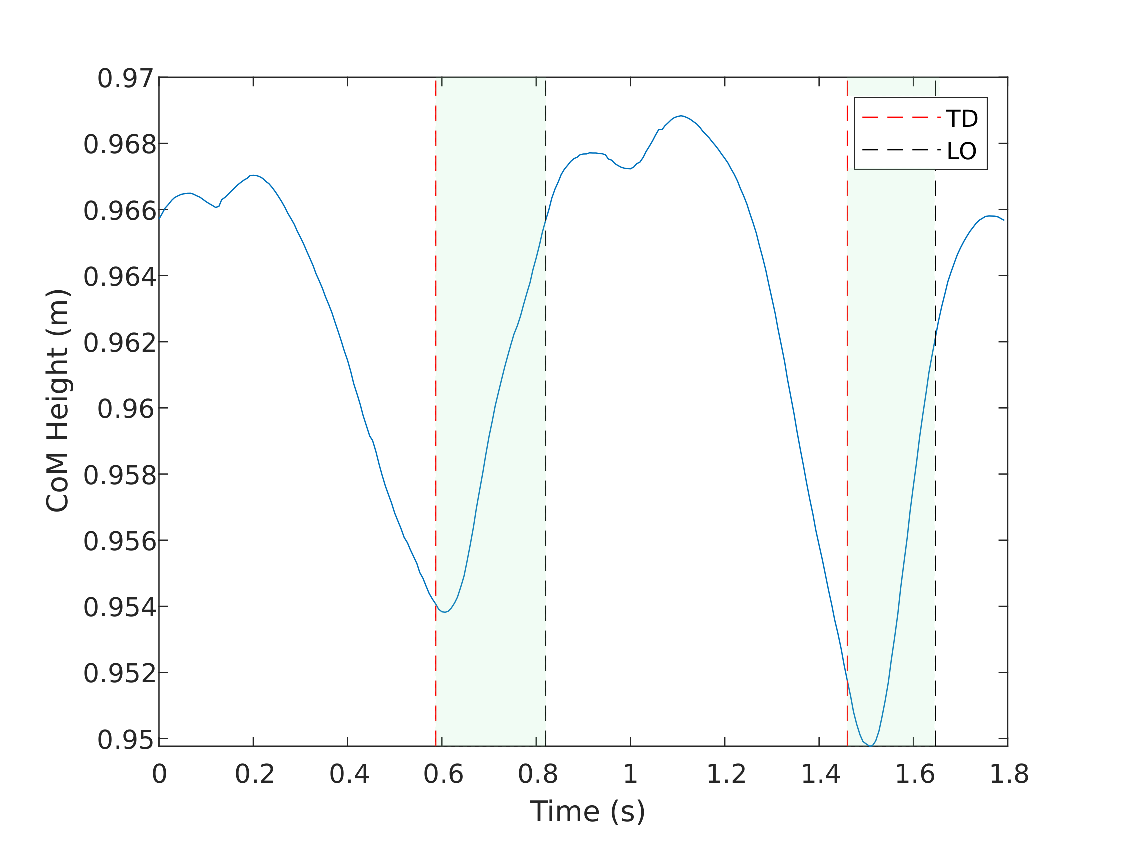
\includegraphics[width=\linewidth]{experimentalCoM.eps}}%
	\hfill
	\subcaptionbox{Vertical excursion of the \com~ of a 2D B-SLIP gait \label{fig:model_traj}}[0.49\textwidth]{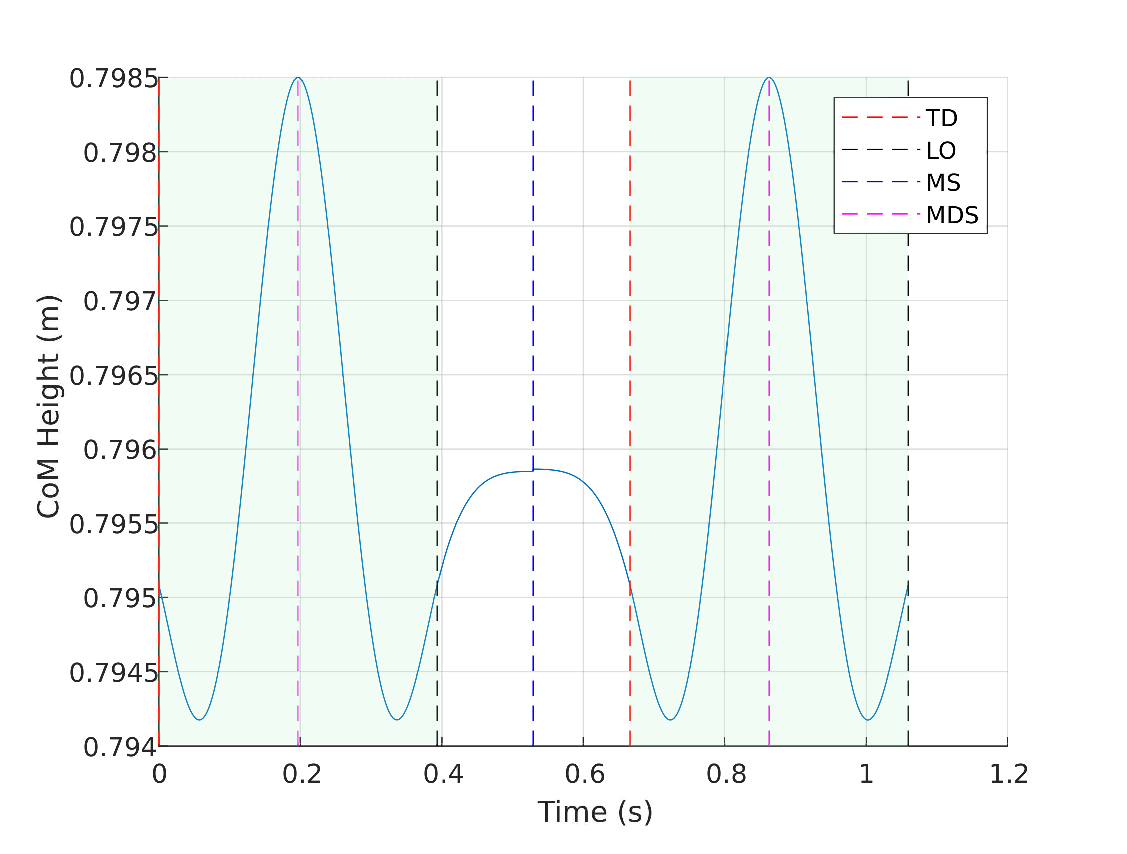
\includegraphics[width=\linewidth]{dSLIP.eps}}%
	\caption{Oscillations during the double-support (shaded green) of 2D B-SLIP gaits at low velocity} \label{fig:traj_compare}
\end{figure}

In their basic forms, the IP, SLIP, and B-SLIP models all ignore lateral dynamics, however, lateral dynamics become more dominant for low-speed gaits. For example, according to the human walking data presented by Fukuchi et al.~\cite{fukuchi2018public}, the peak-to-peak amplitude of the lateral sway of the CoM is approximately 3 cm while walking at 1.27 m/s, but it rises to 9 cm while walking at 0.44 m/s. The model presented by Geyer is defined in only two dimensions, but it generalizes to 3D~\cite{liu2015dynamic,liu2016terrain}. This 3D model allows the lateral sway, which is important while studying low-speed walking, to be taken into consideration. The  oscillations during double support are also eliminated using this model. With appropriate leg length and step width, the sway seen in the gaits generated using the 3D B-SLIP model is comparable to human data. %Considering the lateral sway is especially important while studying walking at low speeds. 

\subsection{Actuated models}

Another approach to gait modeling is including a control input to achieve the desired gait. An example of this approach is the Variable-SLIP (V-SLIP) model, which uses variable stiffness actuation to modulate leg stiffness, in contrast to the original B-SLIP model, which has constant leg stiffness. This model produces a gait that is robust to disturbances, and whose cost of transport are comparable to human walking\footnote{Cost of transport quantifies the energy efficiency of a system; it measures the energy expended to travel a specified distance.}~\cite{visser2017bipedal}. Another approach is the Variable-Height Inverted Pendulum model, in which the CoM height is changed by applying a force along the leg~\cite{koolen2016balance} instead of varying leg stiffness. While all the previously described models have nonlinear dynamics, Kajita et al.~\cite{kajita1991study} proposed a model called the Linear Inverted Pendulum~(LIP) model in which the application of a constrained control input linearizes the dynamics of the system where the height of the \com~ is specified. The LIP model also allows the use of ankle torques to improve model performance on rugged terrain, and it has been extended to three dimensions with the 3D-LIP model~\cite{kajita20013d}.

Actuated models provide a more flexible framework to estimate gait, but determining the control parameters when applying those models to humans becomes a challenge. Therefore, active models are more suited to prosthetic devices which are used in series with the user or legged robots. Most active models have been proposed in regards to legged robots where the dynamics of the robot are well known to the designers. This allows for the complexity of the model to be matched to the complexity of the system dynamics. In the case of exoskeletons, the dynamics of the human body and a human's internal control system are still a subject of study \cite{wolpert1998internal, dounskaia2005internal, kording2007decision}, and they are further complicated by the parallel operation with the exoskeleton suit due to coupling in the human and robot. The simplicity of passive models and the lack of a need to make assumptions about the inputs from a user working in parallel makes them more suited for parallel robots such as exoskeletons. As a result, passive models may be better suited for use in intent detection frameworks. 

\section{The B-SLIP model}\label{sec:bslip_model}
The work presented herein is focused on individuals recovering from iSCIs whose walking velocities were as low as 0.5 m/s. A majority of the duration of steps at low velocities is spent in double support, and it is important to use a model that can describe this gait phase. Therefore, this work considers a passive model, the 3D~B-SLIP model, shown in Fig~\ref{fig:slip}, to model human locomotion. In this model, the \COM~is loaded onto two massless spring legs of length $ l_o $ and stiffness $ k $. The state vector $ \x_{c} $ contains the position and velocity of the CoM, modeled by the point mass $ m $, relative to the stance foot such that $ \x_{c} = [x_{c} ,y_{c} ,z_{c} ,\dot{x}_{c} ,\dot{y}_{c} ,\dot{z}_{c}]^T $. The position of the leading leg at touchdown is given by two angles, the angle between the leading leg and vertical $ \theta $ and the angle $ \varphi $ between the forward axis $ x $  and the ground projection of the leading leg.
%
\begin{figure}
	\centering
	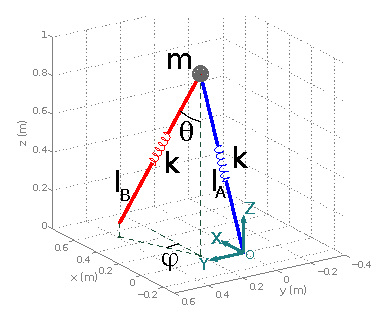
\includegraphics[width=0.6\linewidth]{3DSLIP.eps}
	\caption[The Bipedal Spring Loaded Inverted Pendulum]{The Bipedal Spring Loaded Inverted Pendulum \cite{liu2015dynamic} model of walking}\label{fig:slip}
\end{figure}
%

A gait of the B-SLIP model, as viewed in the sagittal plane\footnote{The sagittal plane is the plane that divides the body into right and left parts.}, is illustrated in Fig.~\ref{fig:slip_gait}. This gait starts at midstance (MS), where the CoM is loaded onto the trailing leg in single-support (SS1). The gait then proceeds with the touchdown~(TD) of the leading leg and enters the double support (DS) phase. The DS phase ends with lift-off~(LO) of the trailing leg and the model enters the second single-support phase~(SS2). The SS2 phase ends in MS, again with the CoM loaded onto the leading leg. As there are alternating SS and DS phases, the dynamics of the B-SLIP model are hybrid.

\begin{figure}
	\centering
	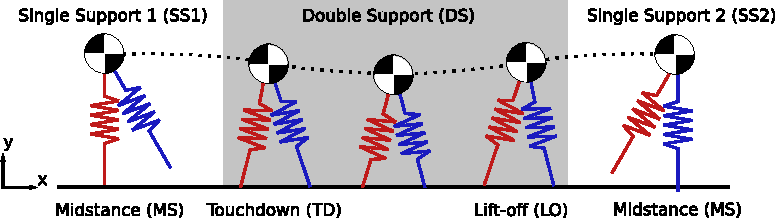
\includegraphics[width=0.9\linewidth]{slip_gait.pdf}
	\caption{One step of a B-SLIP gait}\label{fig:slip_gait}
\end{figure} 

\subsection{Hybrid dynamics of the B-SLIP model}
The dynamics of the model in single support are described by
\begin{equation}
	m\ddot{\p}_{c} = k(l_0 - \lVert \mathbf{l}_i \rVert)\hat{\mathbf{l}}_i + m \mathbf{g}
\end{equation}
\noindent where $ i = \{A,B\} $ denotes the supporting leg, $ \mathbf{l}_i \in \mathbb{R}^3 $ is the vector along the leg from the mass to the position of the stance foot $\p_i$ , $ \hat{\mathbf{l}}_i \in \mathbb{R}^3$ is a unit vector along the leg, and $ \mathbf{g} \in \mathbb{R}^3 $ is the gravity vector. The dynamics during double support are given by
\begin{equation}
	m\ddot{\p}_{c} = k(l_0 - \lVert \mathbf{l}_A \rVert)\hat{\mathbf{l}}_A + k(l_0 - \lVert \mathbf{l}_B \rVert)\hat{\mathbf{l}}_B + m \mathbf{g}
\end{equation}
%
\noindent Certain conditions, known as guards, must be met to enable the switching of the dynamics from one phase to another. There are three switching surfaces to enable phase switches at TD, LO, and MS. These sets are as follows
%
\begin{eqnarray}
	\mathcal{G}_{TD} &=& \{(\p_c,\v_c)| \dot{z}_c < 0 ,z_{c} = z_{T}\} \label{eq:gtd} \\
	\mathcal{G}_{LO} &=& \{(\p_c,\v_c)| \dot{z}_c > 0 ,\lVert \mathbf{l}_A \rVert = l_0\} \label{eq:glo} \\
	\mathcal{G}_{MS} &=& \{(\p_c,\v_c)| \dot{z}_c = 0 ,z_{c} > z_{T} ,\lVert \mathbf{l}_A \rVert < l_0\} \label{eq:gms} 
\end{eqnarray} 
%
\noindent where $ z_{T} = l_0 \cos \theta $ is the threshold height for touchdown. Satisfaction of these guard conditions triggers gait phase switches, and the states of the model are transferred across the switching events using functions called reset maps. For clarity of notation, let $ \z \in \mathbb{R}^{12} $ be the extended state that contains the CoM state and the positions of the feet such that
\[
	\z = \begin{bmatrix}
			\x_{c} \\
			\p_{A} \\
			\p_{B}
	\end{bmatrix}
\]
There are three reset maps following the general form $ \z^+ = h(\z^-,\u) $, where \mbox{$ \u = [\varphi ,\theta ,k]^T $}, and the $ + $ and $ - $ denote pre- and post-switch states. The first map is applied at TD when the guard \eqref{eq:gtd} is satisfied. There are no impacts at touchdown, as spring legs of the B-SLIP model are assumed to be massless so the CoM state remains unchanged, and the position of the leading foot is updated as follows 
%\begin{gather}
%	\mathcal{R}_{TD}:\mathbb{R}^6 \rightarrow \mathbb{R}^6 \nonumber \\ 
%	\mathcal{R}_{TD}(\x^-) = \x^- 
%\end{gather}
\begin{eqnarray}
	\z^+ &=& h_{TD}(\z^-,\u) \qquad h_{TD}:\mathbb{R}^{12}\times \mathbb{R}^{3 }  \rightarrow \mathbb{R}^{12} \\
	{}	&=& \begin{bmatrix}
		\x_{c}^- \\
		\p_{A}^- \\
		h_{TD}^{B}(\p_{c}^-, \u)
	\end{bmatrix} \nonumber
\end{eqnarray}
where
\begin{equation}
	h_{TD}^{B}(\p_{c}^-, \u) = \p_{c}^- + l_0%
	\begin{bmatrix}
		\sin(\theta)\cos(\phi)\\
		\sin(\theta)\sin(\phi)\\
		-\cos(\theta)
	\end{bmatrix}
\end{equation}

\noindent Were the feet assumed to have mass, this reset map would also handle the impact event. The second map is applied as follows when the LO guard \eqref{eq:glo} is satisfied
%
%\begin{gather}
%	\mathcal{R}_{LO}:\mathbb{R}^6 \rightarrow \mathbb{R}^6 \nonumber \\ 
%	\mathcal{R}_{LO}(\x^-) = \x^- \\
%	\p_B \leftarrow \p_A \nonumber
%\end{gather}

\begin{eqnarray}
	\z^+ &=& h_{LO}(\z^-,\u) \qquad h_{LO}:\mathbb{R}^{12} \times \mathbb{R}^{3} \rightarrow \mathbb{R}^{12} \\
	{}	&=& \begin{bmatrix}
		\mathbf{f}(\x_{c}^-,\p_{B}^-) \\
		\p_{B}^- \\
		\p_{A}^-
	\end{bmatrix} \nonumber
\end{eqnarray}
The model uses single-support dynamics after liftoff, so the labels of the foot are switched as the leg that was previously in swing will now be in stance, and the states remain unchanged. Therefore, $ \mathbf{f}(\x_{c}^-,\p_{B}^-) $ computes the lateral position and velocity of the CoM, as the state of the CoM is measured relative to the new stance foot. The last reset map is applied at MS when the guard \eqref{eq:gms} is met.
%
\begin{eqnarray}
	\z^+ &=& h_{MS}(\z^-,\u) \qquad h_{MS}:\mathbb{R}^{12}\times  \mathbb{R}^{3} \rightarrow \mathbb{R}^{12} \\
	{}	&=& \begin{bmatrix}
		\x_{c}^- \\
		\p_{A}^- \\
		\p_{B}^-
	\end{bmatrix} \nonumber
\end{eqnarray}
%
%\begin{equation}
%	\mathcal{R}_{MS}:\x^- \rightarrowtail \p_{CoM} \leftarrow \x_{CoM} - \x_A :\mathbb{R}^6 \rightarrowtail \mathbb{R}^6
%\end{equation}
%
Thus, the B-SLIP model can exhibit periodic gaits by alternately switching through SS and DS phases.

As the B-SLIP model is passive, it does not have any active control inputs to modify gaits and maintain periodicity. Therefore, optimization methods can be used to find periodic model gaits \cite{strogatz2018nonlinear,garcia1998simplest}.

\section{Poincar\'e maps}

Poincar\'e maps are used to study state flows near periodic orbits \cite{strogatz2018nonlinear}. Consider a system whose dynamics are $ \dot{\x} = f(\x) $ where $ \x \in \mathbb{R}^n $. Then a  Poincar\'e section for this system is a set with dimension of $ n-1 $ such that all trajectories passing through the section are transverse to it. It may be placed at a gait event such as MS, TD, or LO when the value of one of the states may be known, i.e., when a guard condition is met. Let the Poincar\'e section be placed at MS, let $ \x_k $ be the state at the $ k^{th} $ crossing of the section, and let $ \mathcal{P}(\x_k) $ be a function that returns the state after one cycle, or a step in the case of the B-SLIP, such that $ \x_{k+1} = \mathcal{P}(\x_k) $. The function $ \mathcal{P}(\x_k) $ is the Poincar\'e map formed by following trajectories from one intersection with the Poincar\'e section to the next, i.e., the Poincar\'e map takes a state on the Poincar\'e section and maps it back onto the section. There may exist an initial state, called a fixed point, representing a periodic orbit where the initial state maps back to itself after one period such that $ \x_k = \mathcal{P}(\x_k) $. 

Studying the behavior of the Poincar\'e maps simplifies a problem about periodic orbits to a problem about the fixed points of a map. Finding analytical solutions for $ \mathcal{P}(\x_k) $ may be difficult, so numerical methods are often used. A Poincar\'e section placed at MS is shown in blue in Fig.~\ref{fig:poincare}. The dynamics of the model are integrated for one step using $ \x_k $ as the initial condition. Optimization methods are used to find initial conditions that yield periodic gaits by minimizing the norm of $ \delta \x $, the error between $ \x_k $ and $ \x_{k+1} $. The nonlinear return map may be linearized about these periodic gaits for further refining the gait search as described in Chapter~\ref{chapter:IMM}. Model gaits for various velocities may be used as references while estimating an exoskeleton user's desired gait by comparing them with measurements of quantities such as \COM~height and velocity using state estimation tools such as the Kalman filter. 

\begin{figure}
	\centering
	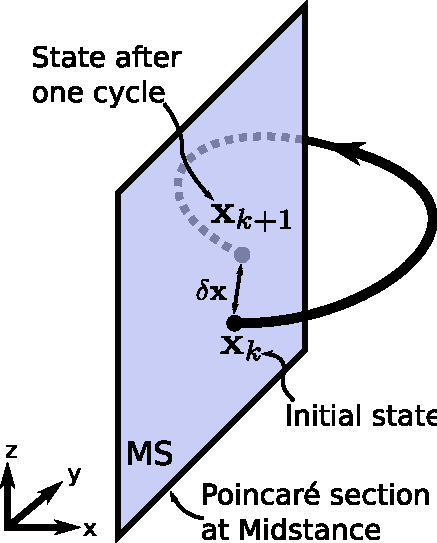
\includegraphics[width=.4\linewidth]{poincare.pdf}
	\caption{A Poincar\'e map used to find periodic gaits}\label{fig:poincare}
\end{figure}

\section{State estimation using Kalman Filters}\label{sec:estimation}

Kalman filtering is a feedback-based sequential optimal estimation technique \cite{kalman1960new} to estimate states and parameters of dynamical systems. The estimates made by a Kalman filter are conditioned on certain measurements of either the states themselves or other quantities that may be represented as functions of the states through a measurement model. State estimation is reliant on these measurements to get a picture of the real world; however, these measurements are rarely free of noise that may adversely affect the quality of the estimates. 

Kalman filters follow a predictor-corrector scheme in which states are propagated using a model of system dynamics which may be incomplete, and stochastic. These states are then corrected using the residual between sensor measurements and the predictions. If the feedback gain applied to this residual is too low, state estimates will not be appropriately corrected, and if the gain is too high, sensor noise will overshadow the system dynamics, and the estimates will begin tracking noise. Kalman filtering presents an optimal method of computing feedback gains that account for modeling and measurement errors with a fundamental assumption that any modeling or measurement errors are zero-mean Gaussian noise processes. The filter was originally proposed for discrete-time linear systems \cite{kalman1960new}. 
 
\subsection{Discrete-time Kalman Filter}
The filter is initialized at a certain initial state estimate $ \xh_0 $ that may have associated uncertainty due to measurement errors. The evolution of this state is described using dynamical system 
%
\begin{eqnarray}
	\x_{k+1} &=& \A_k \x_k + \B_k \u_k + \mathbf{G}_k \mathbf{w}_k,\quad \mathbf{w}_k \sim \mathcal{N}(0, \Q_k) \label{eq:sys_disc}  \\
	\yt_k &=& \H_k \x_k + \mathbf{v}_k,\quad \mathbf{v}_k \sim \mathcal{N}(0,\R_k) \label{eq:meas_lin}
\end{eqnarray}
%
\noindent where $ \x_k $ and $ \u_k $ are the discrete-time states and inputs, $ \y_k $ are the discrete-time measurements, $ \A_k $, $ \B_k $, $ \mathbf{G}_k $, and $ \H_k $ are the system, input, process noise, and measurement models, respectively. The system is assumed to have zero-mean Gaussian noises for process noise $ \mathbf{w}_k $ and measurement noise $ \mathbf{v}_k $ with covariances  $ \Q_k $ and $ \R_k $, respectively. The measurement noise $ \mathbf{v}_k $ is combined with the measurement equation $ \H_k \x_k$ to form the noisy measurement $ \yt_k $. 
%
\begin{figure}
	\centering
	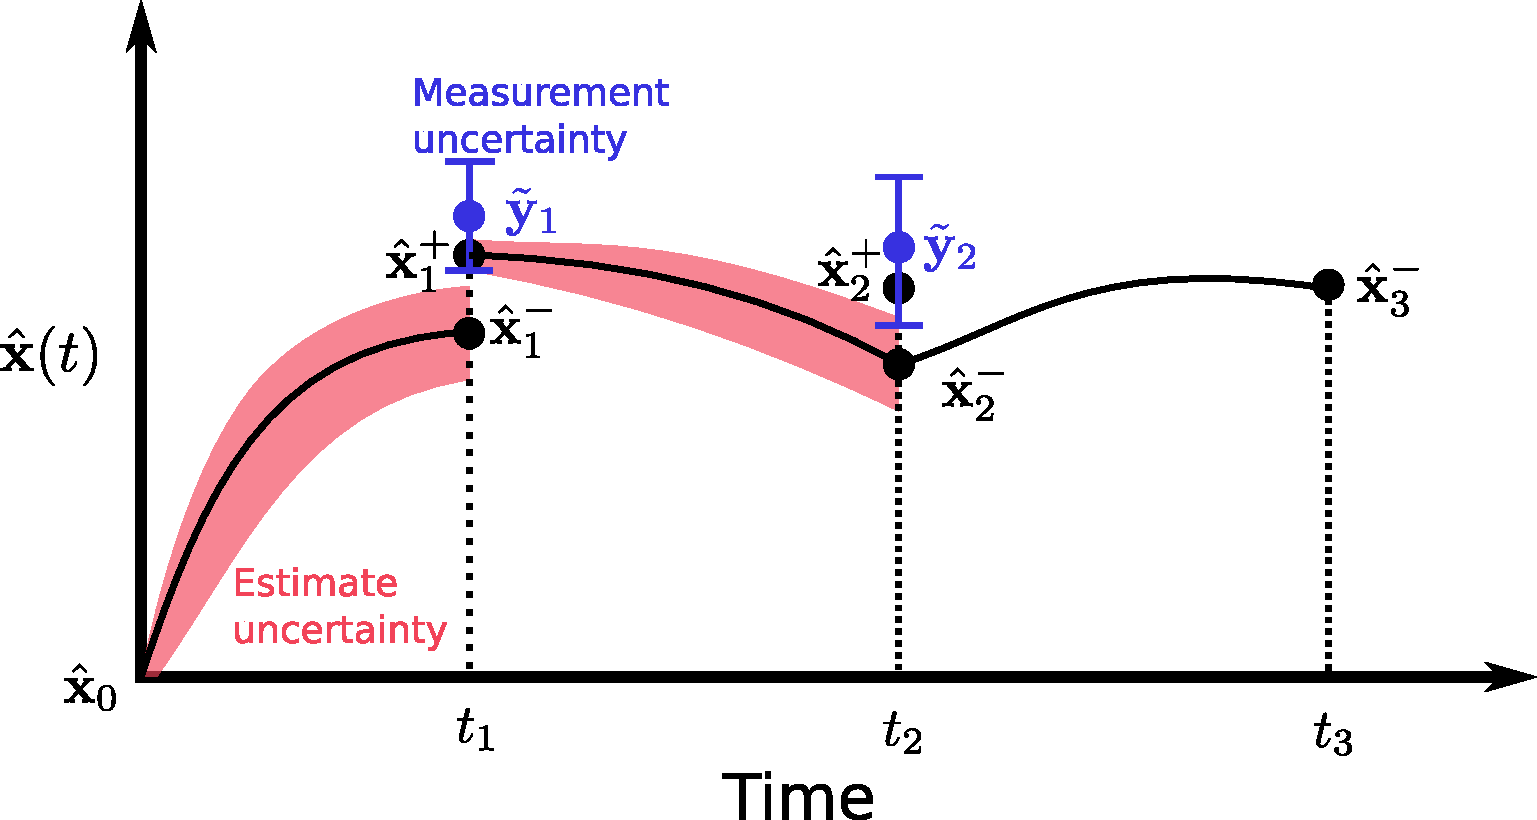
\includegraphics[width=0.85\linewidth]{kalman.pdf}
	\caption{Illustration of the Kalman Filtering process}\label{fig:kalman}
\end{figure}
%

The uncertainty associated with the estimates increases as the state is propagated forward through time using the system dynamics. Regular measurements of state variables are used to update the state estimates and reduce the uncertainty. This process is illustrated in Fig.~\ref{fig:kalman}, where the $ + $ and $ - $ in the superscript denote pre- and post-update states. The system illustrated here is discrete; however, a continuous state evolution is shown to better illustrate the growth in uncertainty. Kalman filters account for the uncertainty in both, the state estimates and the measurements. Further details of this process are as follow. The state estimates and estimate covariance $ \P $ are propagated in discrete time such that
\begin{eqnarray}
	\xh_{k+1} &=& \A_k \xh_k + \B_k \u_k \\
	\P_{k+1} &=& \A_k\P_k \A_k^T + \mathbf{G}_k\Q_k\mathbf{G}_k^T 
\end{eqnarray}
\noindent The states are sequentially updated such that
\begin{eqnarray}
	\K_k &=& \P_k^- \H^T_k \left[\H_k \P_k^- \H^T_k + \R_k\right]^{-1} \label{eq:kalmanGain} \\
	\xh_k^+ &=& \xh_k^- + \K_k[\yt_k- \H_k \xh_k^-)] \label{eq:ekfStateUp} \\
	\P_k^+ &=& [\mathbf{I} - \K_k \H_k]\P_k^-\label{eq:ekfCovUp}
\end{eqnarray}
%
\noindent where the updated estimates, their covariance and the Kalman gain are $ \mathbf{x}_k^+ $, $ \mathbf{P}_k^+ $, and $ \K_k $, respectively. The Kalman gain is optimal, and the error dynamics of the filter are shown to be stable \cite{Crassidis} using the Lyapunov candidate function $ V_k(\e_k) = \e_k^T \P_k^{-1} \e_k $, where $ \e_k \equiv \xh_k - \x_k $. The filter as described above is defined for linear systems, and it has been extended to nonlinear systems.

\subsection{Extended Kalman Filter}
Simple models used to describe legged locomotion have nonlinear dynamics, and so a variation of the Kalman filter named the Extended Kalman Filter (EKF) can be used for these systems. The nonlinear dynamics are linearized about the state estimate to work around the nonlinearity. As this linearization is an approximation of the dynamics, the EKF is not optimal like the discrete-time Kalman filter described previously. Despite the lack of optimality, EKFs have been in widespread use for nonlinear systems \cite{Crassidis, auger2013industrial}. Since most nonlinear dynamics are given in continuous time, a variation of the EKF called the Continuous-Discrete EKF may be used. In this variation, dynamics evolve in continuous time, and measurements are modeled in discrete time. This combination is used for estimation in the work presented herein as it most closely reflects the model and measurement conditions observed in the estimation problem being studied. The general structure of the EKF is similar to the filter presented previously, except the equations are nonlinear as seen by comparing~\eqref{eq:sys_disc} and \eqref{eq:sys}. Consider the following nonlinear dynamical system
% Continuous-Discrete EKF
%
\begin{eqnarray}
	\dot{\x}(t) &=& \mathbf{f}(\x(t),\u(t),\mathbf{w}(t),t),\quad \mathbf{w}(t) \sim \mathcal{N}(0, \Q(t))  \label{eq:sys}  \\
	\yt_k &=& \mathbf{h}(\x_k) + \mathbf{v}_k,\quad \mathbf{v}_k \sim \mathcal{N}(0,\R_k) \label{eq:meas}
\end{eqnarray}
%
\noindent where $ \x(t) $ and $ \u(t) $ are the continuous-time states and inputs, $ \y_k $ are the discrete-time measurements, and $ \mathbf{f}(\x(t),\mathbf{w}(t), \u(t),t) $ and $ \mathbf{h}(\x_k) $ are the system and measurement function, respectively. The system has zero-mean Gaussian process and measurement noises $ \mathbf{w}(t) $ and $ \mathbf{v}_k $, respectively with covariances $ \Q(t) $ and $ \R_k $, respectively. The measurement noise $ \mathbf{v}_k $ is combined with the measurement equation $ \mathbf{h}(\x_k) $ to form the noisy measurement $ \yt_k $. 

The state estimates and estimate covariance $ \P(t) $ are propagated in continuous time such that \vspace{-2em}
\begin{eqnarray}
	\dot{\xh} &=& \mathbf{f}(\xh,\mathbf{w}(t),\u,t) \label{eq:sysProp}\\
	\dot{\P}(t) &=& \F(t)\P(t) + \P(t)\F^T(t) + \mathbf{G}(t)\Q(t)\mathbf{G}(t)^T \label{eq:covProp} \\ 
	\F(t) &\equiv& \frac{\partial \mathbf{f}}{\partial \x} \Bigr |_{\xh(t),\u(t)} \nonumber
\end{eqnarray}

\noindent The states are sequentially updated such that
\begin{eqnarray}
	\K_k &=& \P_k^- \H^T_k(\xh_k^-) \left[\H_k(\xh_k^-)\P_k^- \H^T_k(\xh_k^-) + \R_k\right]^{-1} \\
	\xh_k^+ &=& \xh_k^- + \K_k[\yt_k-\mathbf{h}(\x_k)] \label{eq:sysUp} \\
	\P_k^+ &=& [\mathbf{I} - \K_k \H_k(\xh_k^-)]\P_k^-,\quad \H_k(\xh_k^-) \equiv \frac{\partial \mathbf{h}}{\partial \x} \Bigr |_{\xh_k^-}
\end{eqnarray}
%
\noindent where $ \K_k $ is the Kalman gain, $ \F(t) $, and $ \H_k(\xh_k^-) $ are the linearized dynamics and measurement model, respectively. The updated estimates and their covariance are $ \mathbf{x}_k^+ $ and $ \mathbf{P}_k^+ $, respectively. The above equations describe a Continous-Discrete Kalman filter setup \cite{Crassidis}. System dynamics are propagated in continuous time \eqref{eq:sysProp}, but states are updated in discrete time \eqref{eq:sysUp} since measurements are discrete. This setup handles the nonlinear dynamics of the models used to emulate legged locomotion; however, it does not handle the hybrid nature of these models.

Each step of human walking has alternating single and double support periods depending on how many legs are in contact with the ground. Therefore, in addition to being nonlinear, models of legged locomotion have hybrid dynamics to describe different gait phases, i.e., different dynamics for different phases. The EKF can be used as an estimation tool to handle these hybrid dynamics in a framework known as Interacting Multi-Model (IMM) estimation. This framework allows the use of multiple EKFs in parallel and is discussed in detail in Chapter~\ref{chapter:IMM}.

\section{Exoskeleton data used for testing} \label{sec:exoData}
The estimation schemes presented in this work were all tested on walking trial data of users walking in an EksoGT exoskeleton (Fig.~\ref{fig:exoOperator})
developed by Ekso Bionics. The reliance of many state-of-the-art intent inference approaches on external sensors like electromyography (EMG) may be problematic in practical applications, as EMG sensors need consistency in placement and may slip during usage due to perspiration~\cite{tkach2010study,ison2014role}. Therefore, this work strives to exclusively use measurements from sensors onboard the exoskeleton, as they may offer a more reliable option \cite{Gambon20b}, in addition to being cost-effective. 

\begin{figure}
	\centering
	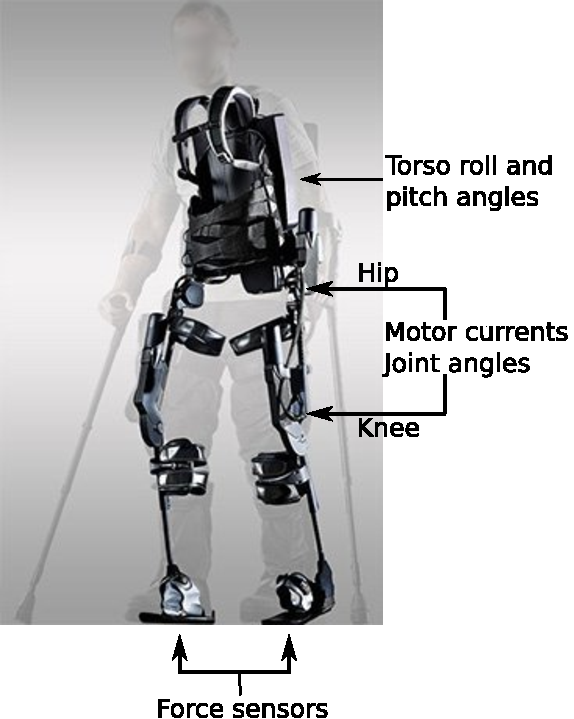
\includegraphics[height=3.5in]{exo_gt.pdf}
	\vspace{-1em}
	\caption[Measurements obtained from sensors onboard the Ekso GT]{Measurements obtained from sensors onboard the Ekso GT \cite{eksoOperator}}\label{fig:exoOperator}
	\vspace{-1em}
\end{figure}

Trial data were collected as part of a study approved by the IRB of the University of Notre Dame (Protocol 18-04-4650) \cite{gambon2020effects}. The exoskeleton has two modes of operation, free and adaptive. Free mode is similar to gravity compensation, whereas in adaptive mode, the exoskeleton follows a predefined trajectory and corrects any deviations from it. This work uses data from trials of three uninjured and two users with iSCI. Uninjured users underwent trials in both modes, and users with iSCI only underwent trials in adaptive mode. One of the users with iSCI, IU-1, had a complete SCI at the middle of the spine (T5), and the second user, IU-2, had an incomplete SCI from the middle to the lower spine (T8 to L2). All users were highly experienced in the use of the EksoGT. The subjects used the exoskeleton at a self-selected speed with the assistance of a walker and were at a steady-state gait before being issued a verbal command to either speed up or slow down. The trial sequence was pseudo-random, and each subject underwent three speed-up (SU) and slow-down (SD) trials for a total of six trials.

Sensors onboard the exoskeleton provide hip pitch, knee pitch, and torso pitch and roll angles\footnote{Pitch angles lie within the sagittal plane, and roll angles lie within the frontal plane. The frontal plane is the vertical plane that runs side-to-side, dividing the body in anterior and posterior portions.}, and are fused to estimate the height and fore-aft position of the hip in a global frame. These readings were used to approximate the location of the subject's CoM with respect to the stance foot. Since the position of the CoM is considered relative to the stance foot, the drift that may be present in the global position estimate has negligible a effect on step-to-step calculations. The subject's height, and thigh and shank lengths were recorded, and the location of their CoM was approximated to be at the centroid of the pelvis. The remaining dimensions such as ankle height and hip-width were computed using anthropometry relationships defined by Winter \cite{winter2009biomechanics}. The CoM velocities and angular velocities of the joints and torso were computed with finite-difference approximations as direct gyro measurements were not accessible. Gait events identified for the estimator were MS, TD, and LO. A zero-crossing event between the left and right hip angles reported by the exoskeleton was used to detect MS. TD was detected when force sensor readings from both feet were above a threshold of 5\% of the maximum sensor value, and LO was detected when the reading from the trailing foot fell below this threshold. 

\section{Summary}
This chapter serves as a repository of background information to help focus the subsequent chapters on their corresponding contributions. Poincar\'e maps were used during the generation of a library containing gaits of the B-SLIP model. This library is used in the IMM framework for gait phase and velocity estimation as described in Chapter~\ref{chapter:IMM}. Kalman filters along with a Bayesian update stage form the basis of the estimators used in Chapters~\ref{chapter:BKF}~and~\ref{chapter:MP}. The IMM framework was tested on synthetic data from simulated library gaits and on the exoskeleton trial data described in Section \ref{sec:exoData}. The estimators used in Chapters~\ref{chapter:BKF}~and~\ref{chapter:MP} were tested solely on exoskeleton data.
